\documentclass[fleqn,12pt]{SelfArx}
\setlength{\columnsep}{0.55cm} % Distance between the two columns of text
\setlength{\fboxrule}{0.75pt} % Width of the border around the abstract
\definecolor{color1}{RGB}{0,0,90} % Color of the article title and sections
\definecolor{color2}{RGB}{0,20,20} % Color of the boxes behind the abstract and headings
\usepackage{hyperref} % Required for hyperlinks
\usepackage{multicol}
\hypersetup{hidelinks,colorlinks,breaklinks=true,urlcolor=color2,citecolor=color1,linkcolor=color1,bookmarksopen=false,pdftitle={Title},pdfauthor={Author}}
\def\mystyle{decsci}
\usepackage{mathtools} 
\usepackage{amssymb}

\title{Bibliography style = \mystyle}
\date{}

\JournalInfo{Project 2018-19 Term 2} % Journal information
\PaperTitle{QF620 - Stochastic Modelling in Finance} % Article title
\Authors{Kim Chan Jung\textsuperscript{1}, Tang Hong Yuan Xavier\textsuperscript{2}, Chen Qi Zhao Brandon\textsuperscript{3}, Jin Weiguo Mark\textsuperscript{4}, Harish Reddy\textsuperscript{5}} % Authors

\Abstract{This report encapsulates the fundamentals of Stochastic Modelling in a condensed report by applying theories including but not limited to, Black Scholes model, Bachelier model, Black76 model, Displaced-diffusion model. Through the application of computational and programming methodologies, the team managed to construct the various models and calibrate them to match the option prices. Using the output generated from the various models, the team analysed the results and elaborated on its underlying significance.}

\begin{document}
\maketitle
\thispagestyle{empty} % Removes page numbering from the first page


\section{Analytical Option Formulae}
\subsection{Black-Scholes Vanilla Call Option}

The Black-Scholes model for the stock price process is defined as
$$
dS_t = rS_tdt + \sigma S_tdW_t
$$

By solving the stochastic differential equation using It\^{o}'s formula, we can get
$$
S_t = S_0e^{\big(r-\frac{\sigma^2}{2}\big)T+\sigma W_t}
$$

Vanilla European call option price is derived as below.
$$
V_o^{c} = e^{-rT}{E}[(S_t-K)^{+}]
$$
$$
= e^{-rT}\frac{1}{\sqrt{2\pi}}\int_{-\infty}^{\infty}(S_0e^{\big(r-\frac{\sigma^{2}}{2}\big)T +\sigma\sqrt{T}x}-K)^{+}e^{-\frac{x^{2}}{2}}dx
$$
Here, 
$$S_0e^{\big(r-\frac{\sigma^{2}}{2}\big)T +\sigma\sqrt{T}x} > K$$
$$ 
x > \frac{\log({\frac{K}{S_0}})-\big(r-\frac{\sigma^{2}}{2}\big)T}{\sigma\sqrt{T}} = x^{*}
$$
Then,
$$
= e^{-rT}\frac{1}{\sqrt{2\pi}}\Bigg[S_0e^{\big(r-\frac{\sigma^{2}}{2}\big)T}\int_{x^{*}}^{\infty}e^{\sigma\sqrt{T}x}e^{-\frac{x^{2}}{2}}dx - K\int_{x^{*}}^{\infty}e^{-\frac{x^{2}}{2}}dx\Bigg]
$$$$
= e^{-rT}\Bigg[S_0e^{\big(r-\frac{\sigma^{2}}{2}\big)T}\frac{1}{\sqrt{2\pi}}\int_{x^{*}}^{\infty}e^{-\frac{x^{2}-2\sigma\sqrt{T}x+\sigma^{2}T-\sigma^{2}T}{2}}dx -
$$$$
K\Phi(-x^{*})\Bigg]
$$$$
= S_0\frac{1}{\sqrt{2\pi}}\int_{x^{*}}^{\infty}e^{-\frac{(x-\sigma\sqrt{T})^{2}}{2}}dx - Ke^{-rt}\Phi(-x^{*})
$$
Let 
$$y = x-\sigma\sqrt{T} \Rightarrow dy=dx$$
$$x = x^{*}, y = x^{*}-\sigma\sqrt{T}$$
Then,
$$
V_o^{c} = S_0\frac{1}{\sqrt{2\pi}}\int_{x^{*}-\sigma\sqrt{T}}^{\infty}e^{-\frac{y^{2}}{2}}dy - Ke^{-rT}\Phi(-x^{*})
$$
$$
= S_0\Phi(-x^{*}+\sigma\sqrt{T}) - Ke^{-rT}\Phi({-x^{*}})
$$$$
V_o^{c} = S_0\Phi\Bigg(\frac{\log({\frac{S_0}{K}})+(r+\frac{\sigma^{2}}{2})T}{\sigma\sqrt{T}}\Bigg) -
$$$$
Ke^{-rT}\Phi\Bigg(\frac{\log({\frac{S_0}{K}})+\big(r-\frac{\sigma^{2}}{2}\big)T}{\sigma\sqrt{T}}\Bigg)
$$

\subsection{Black-Scholes Vanilla Put Option}
$$
V_o^{p} = e^{-rT}{E}[(K-S_t)^{+}]
$$$$
= e^{-rT}\frac{1}{\sqrt{2\pi}}\int_{-\infty}^{\infty}(K-S_0e^{\big(r-\frac{\sigma^{2}}{2}\big)T +\sigma\sqrt{T}x})^{+}e^{-\frac{x^{2}}{2}}dx
$$
Here, 
$$S_0e^{\big(r-\frac{\sigma^{2}}{2}\big)T +\sigma\sqrt{T}x} < K$$
$$ 
x < \frac{\log({\frac{K}{S_0}})-\big(r-\frac{\sigma^{2}}{2}\big)T}{\sigma\sqrt{T}} = x^{*}
$$
Then,
$$
V_o^{p} = e^{-rT}\frac{1}{\sqrt{2\pi}}\int_{-\infty}^{x^{*}}\Big(K-S_0e^{\big(r-\frac{\sigma^{2}}{2}\big)T +\sigma\sqrt{T}x}\Big)e^{-\frac{x^{2}}{2}}dx
$$$$
= e^{-rT}K\frac{1}{\sqrt{2\pi}}\int_{-\infty}^{x^{*}}e^{-\frac{x^{2}}{2}}dx-
$$$$
e^{-rT}S_0\frac{1}{\sqrt{2\pi}}\int_{-\infty}^{x^{*}}e^{\big(r-\frac{\sigma^{2}}{2}\big)T+\sigma\sqrt{T}x}e^{-\frac{x^{2}}{2}}dx
$$$$
=e^{-rT}K\Phi(x^{*})-S_0e^{-\frac{1}{2}\sigma^{2}T}\frac{1}{\sqrt{2\pi}}\int_{-\infty}^{x^{*}}e^{\sigma\sqrt{T}x}e^{-\frac{x^{2}}{2}}dx
$$$$
=e^{-rT}K\Phi(x^{*})-S_0\frac{1}{\sqrt{2\pi}}\int_{-\infty}^{x^{*}}e^{-\frac{(x-\sigma\sqrt{T})^{2}}{2}}dx
$$
Let 
$$y = x-\sigma\sqrt{T} \Rightarrow dy=dx$$
$$x = x^{*}, y = x^{*}-\sigma\sqrt{T}$$
Then,
$$
V_o^{p} = e^{-rT}K\Phi(x^{*}) - S_0\frac{1}{\sqrt{2\pi}}\int_{-\infty}^{x^{*}-\sigma\sqrt{T}}e^{-\frac{y^{2}}{2}}dy
$$$$
= e^{-rT}K\Phi(x^{*}) - S_0[\Phi(x^{*}-\sigma\sqrt{T})]
$$$$
V_o^{p} = e^{-rT}K\Phi\Bigg(\frac{\log({\frac{K}{S_0}})-\big(r-\frac{\sigma^{2}}{2}\big)T}{\sigma\sqrt{T}}\Bigg) -
$$$$
S_0\Phi\Bigg(\frac{\log({\frac{K}{S_0}})-(r+\frac{\sigma^{2}}{2})T}{\sigma\sqrt{T}}\Bigg)
$$

\subsection{Black-Scholes Digital Cash-or-Nothing Call}
$$
V^{c}_{Cash Digital}(0) = e^{-rT}\frac{1}{\sqrt{2\pi}}\int_{-\infty}^{\infty}\mathbf{1}_{S_T>K}e^{-\frac{x^{2}}{2}}dx
$$
$$
= e^{-rT}\frac{1}{\sqrt{2\pi}}\int_{x^{*}}^{\infty}e^{-\frac{x^{2}}{2}}dx
$$
where,
$$
x^{*} = \frac{\log({\frac{K}{S_0}})-\big(r-\frac{\sigma^{2}}{2}\big)T}{\sigma\sqrt{T}} 
$$
Therefore,
$$
V^{c}_{Cash Digital}(0) = e^{-rT}\Phi\Bigg(\frac{\log({\frac{S_0}{K}})+\big(r-\frac{\sigma^{2}}{2}\big)T}{\sigma\sqrt{T}} \Bigg)
$$

\subsection{Black-Scholes Digital Cash-or-Nothing Put}
$$
V^{p}_{Cash Digital}(0) = e^{-rT}\frac{1}{\sqrt{2\pi}}\int_{-\infty}^{\infty}\mathbf{1}_{K>S_T}e^{-\frac{x^{2}}{2}}dx
$$
$$
= e^{-rT}\frac{1}{\sqrt{2\pi}}\int_{-\infty}^{x^{*}}e^{-\frac{x^{2}}{2}}dx
$$
where,
$$
x^{*} = \frac{\log({\frac{K}{S_0}})-\big(r-\frac{\sigma^{2}}{2}\big)T}{\sigma\sqrt{T}} 
$$
Therefore,
$$
V^{p}_{Cash Digital}(0) = e^{-rT}\Phi\Bigg(\frac{\log({\frac{K}{S_0}})-\big(r-\frac{\sigma^{2}}{2}\big)T}{\sigma\sqrt{T}} \Bigg)
$$

\subsection{Black-Scholes Digital Asset-or-Nothing Call}
$$
V^{c}_{Asset Digital}(0) = e^{-rT}\frac{1}{\sqrt{2\pi}}\int_{-\infty}^{\infty}S_T\mathbf{1}_{S_T>K}e^{-\frac{x^{2}}{2}}dx
$$
$$
= e^{-rT}\frac{1}{\sqrt{2\pi}}\int_{x^{*}}^{\infty}S_Te^{-\frac{x^{2}}{2}}dx
$$
where,
$$
x^{*} = \frac{\log({\frac{K}{S_0}})-\big(r-\frac{\sigma^{2}}{2}\big)T}{\sigma\sqrt{T}} 
$$
Therefore,
$$
V^{c}_{Asset Digital}(0) = e^{-rT}\frac{1}{\sqrt{2\pi}}\int_{x^{*}}^{\infty}S_0e^{\big(r-\frac{\sigma^{2}}{2}\big)T +\sigma\sqrt{T}x}e^{-\frac{x^{2}}{2}}dx
$$
From the same process as Black-Scholes vanilla call option,
$$
 V^{c}_{Asset Digital}(0) = S_0\Phi\Bigg(\frac{\log({\frac{S_0}{K}})+(r+\frac{\sigma^{2}}{2})T}{\sigma\sqrt{T}} \Bigg)
$$

\subsection{Black-Scholes Digital Asset-or-Nothing Put}
$$
V^{p}_{Asset Digital}(0) = e^{-rT}\frac{1}{\sqrt{2\pi}}\int_{-\infty}^{\infty}S_T\mathbf{1}_{K>S_T}e^{-\frac{x^{2}}{2}}dx
$$
$$
= e^{-rT}\frac{1}{\sqrt{2\pi}}\int_{-\infty}^{x^{*}}S_Te^{-\frac{x^{2}}{2}}dx
$$
where,
$$
x^{*} = \frac{\log({\frac{K}{S_0}})-\big(r-\frac{\sigma^{2}}{2}\big)T}{\sigma\sqrt{T}} 
$$
Therefore,
$$
V^{p}_{Asset Digital}(0) = e^{-rT}\frac{1}{\sqrt{2\pi}}\int_{-\infty}^{x^{*}}S_0e^{\big(r-\frac{\sigma^{2}}{2}\big)T +\sigma\sqrt{T}x}e^{-\frac{x^{2}}{2}}dx
$$
From the same process as Black-Scholes vanilla put option,
$$
V^{p}_{Asset Digital}(0) = S_0\Phi\Bigg(\frac{\log({\frac{K}{S_0}})-(r+\frac{\sigma^{2}}{2})T}{\sigma\sqrt{T}}\Bigg)
$$

\subsection{Bachelier Vanilla Call Option}
The Bachelier model for the stock price process is defined as
$$
dS_t = \sigma S_0dW_t
$$$$
S_T = S_0(1 + \sigma W_T), \qquad \qquad W_T\sim N(0, T)
$$
Vanilla European call option price is derived as below.
$$
V_o^{c} = {E}[(S_t-K)^{+}]
$$$$
= {E}[(S_0(1 + \sigma W_T)-K)^{+}]
$$$$
= {E}[(S_0(1 + \sigma \sqrt{T}x)-K)^{+}],\qquad \qquad X\sim N(0, 1)
$$$$
= \frac{1}{\sqrt{2\pi}}\int_{-\infty}^{\infty}(S_0 + \sigma S_0\sqrt{T}x-K)^{+}e^{-\frac{x^{2}}{2}}dx
$$
Here,
$$
S_0 + \sigma S_0\sqrt{T}x -K>0
$$$$
x > \frac{K-S_0}{\sigma S_0\sqrt{T}} = x^{*}
$$
Then,
$$
V_o^{c} = \frac{1}{\sqrt{2\pi}}\int_{x^{*}}^{\infty}(S_0 + \sigma S_0\sqrt{T}x-K)e^{-\frac{x^{2}}{2}}dx
$$$$
= \frac{1}{\sqrt{2\pi}}\Bigg(\int_{x^{*}}^{\infty}(S_0-K)e^{-\frac{x^{2}}{2}}dx +  \int_{x^{*}}^{\infty} \sigma S_0\sqrt{T}xe^{-\frac{x^{2}}{2}}dx\Bigg)
$$$$
= (S_0-K)\Big[\Phi(\infty)-\Phi(x^{*})\Big] + \frac{1}{\sqrt{2\pi}}\int_{x^{*}}^{\infty}\sigma S_0\sqrt{T}xe^{-\frac{x^{2}}{2}}dx
$$
Let $ u = -\frac{x^{2}}{2} $, $du = -xdx$
$$
V_o^{c}= (S_0-K)\Phi(-x^{*}) - \sigma S_0\sqrt{T}\frac{1}{\sqrt{2\pi}}\int_{x^{*}}^{\infty}e^{u}du
$$$$
= (S_0-K)\Phi(-x^{*}) - \sigma S_0\sqrt{T}\frac{1}{\sqrt{2\pi}}\big[e^{-\frac{x^{2}}{2}}\big]_{x^{*}}^\infty
$$$$
= (S_0-K)\Phi(-x^{*}) + \sigma S_0\sqrt{T}\phi(-x^{*})
$$
$$
= (S_0-K)\Phi\bigg(\frac{S_0-K}{\sigma S_0\sqrt{T}}\bigg) + \sigma S_0\sqrt{T}\phi\bigg(\frac{S_0-K}{\sigma S_0\sqrt{T}}\bigg)
$$

\subsection{Bachelier Vanilla Put Option}
$$
V_o^{p} = {E}[(K-S_t)^{+}]
$$$$
= {E}[(K-S_0(1 + \sigma W_T))^{+}]
$$$$
= {E}[(K-S_0(1 + \sigma \sqrt{T}x))^{+}],\qquad \qquad X\sim N(0, 1)
$$$$
= \frac{1}{\sqrt{2\pi}}\int_{-\infty}^{\infty}(K-S_0 - \sigma S_0\sqrt{T}x)^{+}e^{-\frac{x^{2}}{2}}dx
$$

Here,
$$
K - S_0 - \sigma S_0\sqrt{T}x >0
$$$$
x < \frac{K-S_0}{\sigma S_0\sqrt{T}} = x^{*}
$$
Then,
$$
V_o^{p} = \frac{1}{\sqrt{2\pi}}\int_{-\infty}^{x^{*}}(K-S_0 - \sigma S_0\sqrt{T}x)e^{-\frac{x^{2}}{2}}dx
$$$$
= \frac{1}{\sqrt{2\pi}}\Bigg(\int_{-\infty}^{x^{*}}(K-S_0)e^{-\frac{x^{2}}{2}}dx - \int_{-\infty}^{x^{*}}\sigma S_0\sqrt{T}xe^{-\frac{x^{2}}{2}}dx\Bigg)
$$$$
=(K-S_0)\Phi(x^{*}) - \frac{1}{\sqrt{2\pi}}\int_{-\infty}^{x^{*}}\sigma S_0\sqrt{T}xe^{-\frac{x^{2}}{2}}dx
$$
Let $ u = -\frac{x^{2}}{2} $, $du = -xdx$
$$
V_o^{p} =(K-S_0)\Phi(x^{*}) + \sigma S_0\sqrt{T}\frac{1}{\sqrt{2\pi}}\int_{-\infty}^{x^{*}}e^{u}du
$$$$
= (K-S_0)\Phi(x^{*}) + \sigma S_0\sqrt{T}\frac{1}{\sqrt{2\pi}}\bigg[e^{-\frac{x^{2}}{2}}\bigg]_{-\infty}^{x^{*}}
$$$$
= (K-S_0)\Phi(x^{*}) + \sigma S_0\sqrt{T}\phi(x^{*})
$$
$$
= (K-S_0)\Phi\bigg(\frac{K-S_0}{\sigma S_0\sqrt{T}}\bigg) + \sigma S_0\sqrt{T}\phi\bigg(\frac{K-S_0}{\sigma S_0\sqrt{T}}\bigg)
$$

\subsection{Bachelier Digital Cash-or-Nothing Call Option}
$$
V^{c}_{Cash Digital}(0) = \frac{1}{\sqrt{2\pi}}\int_{-\infty}^{\infty}\mathbf{1}_{S_T>K}e^{-\frac{x^{2}}{2}}dx
$$
$$
= \frac{1}{\sqrt{2\pi}}\int_{x^{*}}^{\infty}e^{-\frac{x^{2}}{2}}dx
$$
where,
$$
x^{*} = \frac{K-S_0}{\sigma S_0\sqrt{T}}
$$
Therefore,
$$
V^{c}_{Cash Digital}(0) = \Phi\bigg(\frac{S_0-K}{\sigma S_0\sqrt{T}}\bigg)
$$

\subsection{Bachelier Digital Cash-or-Nothing Put Option}
$$
V^{p}_{Cash Digital}(0) = \frac{1}{\sqrt{2\pi}}\int_{-\infty}^{\infty}\mathbf{1}_{K>S_T}e^{-\frac{x^{2}}{2}}dx
$$
$$
= \frac{1}{\sqrt{2\pi}}\int_{\infty}^{x^{*}}e^{-\frac{x^{2}}{2}}dx
$$
where,
$$
x^{*} = \frac{K-S_0}{\sigma S_0\sqrt{T}} 
$$
Therefore,
$$
V^{p}_{Cash Digital}(0) = \Phi\bigg(\frac{K-S_0}{\sigma S_0\sqrt{T}}\bigg)
$$
\subsection{Bachelier Digital Asset-or-Nothing Call Option}
$$
V^{c}_{Asset Digital}(0) = \frac{1}{\sqrt{2\pi}}\int_{-\infty}^{\infty}S_T\mathbf{1}_{S_T>K}e^{-\frac{x^{2}}{2}}dx
$$
$$
= \frac{1}{\sqrt{2\pi}}\int_{x^{*}}^{\infty}S_Te^{-\frac{x^{2}}{2}}dx
$$
where,
$$
x^{*} = \frac{K-S_0}{\sigma S_0\sqrt{T}}
$$
Therefore,
$$
V^{c}_{Asset Digital}(0) = \frac{1}{\sqrt{2\pi}}\int_{x^{*}}^{\infty} S_0(1 + \sigma \sqrt{T}x)e^{-\frac{x^{2}}{2}}dx
$$
From the same process as Bachelier vanilla call option,
$$
V^{c}_{Asset Digital}(0) = S_0\Phi\bigg(\frac{S_0-K}{\sigma S_0\sqrt{T}}\Big) + \sigma S_0\sqrt{T}\phi\Big(\frac{S_0-K}{\sigma S_0\sqrt{T}}\bigg)
$$

\subsection{Bachelier Digital Asset-or-Nothing Put Option}
$$
V^{p}_{Asset Digital}(0) = \frac{1}{\sqrt{2\pi}}\int_{-\infty}^{\infty}S_T\mathbf{1}_{K>S_T}e^{-\frac{x^{2}}{2}}dx
$$
$$
= \frac{1}{\sqrt{2\pi}}\int_{\infty}^{x^{*}}S_Te^{-\frac{x^{2}}{2}}dx
$$
where,
$$
x^{*} = \frac{K-S_0}{\sigma S_0\sqrt{T}} 
$$
Therefore,

$$
V^{p}_{Asset Digital}(0) = \frac{1}{\sqrt{2\pi}}\int_{\infty}^{x^{*}} S_0(1 + \sigma \sqrt{T}x)e^{-\frac{x^{2}}{2}}dx
$$
From the same process as Bachelier vanilla put option,
$$
V^{p}_{Asset Digital}(0) = S_0\Phi\bigg(\frac{K-S_0}{\sigma S_0\sqrt{T}}\bigg) + \sigma S_0\sqrt{T}\phi\bigg(\frac{K-S_0}{\sigma S_0\sqrt{T}}\bigg)
$$

\subsection{Black76 Vanilla Call Option}

$$
dF_t = \sigma F_tdW_t
$$$$
F_t = F_0e^{-\frac{\sigma^{2}T}{2} + \sigma W_t}
$$$$
F_0 = S_0e^{rT}
$$
Vanilla European call option price is derived as below.
$$
V_o^{c} = e^{-rT}{E}[(F_t-K)^{+}]
$$$$
= e^{-rT}\frac{1}{\sqrt{2\pi}}\int_{-\infty}^{\infty}(F_0e^{-\frac{\sigma^{2}T}{2} +\sigma\sqrt{T}x}-K)^{+}e^{-\frac{x^{2}}{2}}dx
$$
$$
= e^{-rT}\frac{1}{\sqrt{2\pi}}\int_{-\infty}^{\infty}(S_0e^{\big(r-\frac{\sigma^{2}}{2}\big)T +\sigma\sqrt{T}x}-K)^{+}e^{-\frac{x^{2}}{2}}dx
$$
The result above is exactly same as Black-Scholes model.
Therefore, when we rearrange Black-Scholes model for forward price, we can get Black76 model.

Black-Scholes Model:
$$
V_o^{c} = S_0\Phi\Bigg(\frac{\log({\frac{S_0}{K}})+(r+\frac{\sigma^{2}}{2})T}{\sigma\sqrt{T}}\Bigg) -
$$$$
Ke^{-rT}\Phi\Bigg(\frac{\log({\frac{S_0}{K}})+\big(r-\frac{\sigma^{2}}{2}\big)T}{\sigma\sqrt{T}}\Bigg)
$$
Black76 Model:
$$
V_o^{c} = e^{-rT}\Bigg[ F_0\Phi\Bigg(\frac{\log({\frac{F_0}{K}})+\frac{1}{2}\sigma^{2}T}{\sigma\sqrt{T}}\Bigg) -
$$$$
K\Phi\Bigg(\frac{\log({\frac{F_0}{K}})-\frac{1}{2}\sigma^{2}T}{\sigma\sqrt{T}}\Bigg)\Bigg]
$$

\subsection{Black76 Other options}
As shown in Black76 Vanilla call option, when we rearrange Black-Scholes models for forward price, we can get Black76 model.
\\
\\
Black76 Vanilla Put Option :
$$
V_o^{p} =
$$$$
e^{-rT}K\Phi\Bigg(\frac{\log({\frac{K}{S_0}})-\big(r-\frac{\sigma^{2}}{2}\big)T}{\sigma\sqrt{T}}\Bigg) -
$$$$
S_0\Phi\Bigg(\frac{\log({\frac{K}{S_0}})-(r+\frac{\sigma^{2}}{2})T}{\sigma\sqrt{T}}\Bigg)
$$
$$
= e^{-rT}\Bigg[K\Phi\Bigg(\frac{\log({\frac{K}{F_0}})+\frac{1}{2}\sigma^{2}T}{\sigma\sqrt{T}}\Bigg) - F_0\Phi\Bigg(\frac{\log({\frac{K}{F_0}})-\frac{1}{2}\sigma^{2}T}{\sigma\sqrt{T}}\Bigg)\Bigg]
$$
Black76 Digital Cash-or-Nothing Call Option :
$$
V^{c}_{Cash Digital}(0) = e^{-rT}\Phi\Bigg(\frac{\log({\frac{S_0}{K}})+\big(r-\frac{\sigma^{2}}{2}\big)T}{\sigma\sqrt{T}} \Bigg)
$$
$$
= e^{-rT}\Phi\Bigg(\frac{\log({\frac{F_0}{K}})-\frac{1}{2}\sigma^{2}T}{\sigma\sqrt{T}} \Bigg)
$$
Black76 Digital Cash-or-Nothing Put Option :
$$
V^{p}_{Cash Digital}(0) = e^{-rT}\Phi\Bigg( \frac{\log({\frac{K}{S_0}})-\big(r-\frac{\sigma^{2}}{2}\big)T}{\sigma\sqrt{T}} \Bigg)
$$
$$
= e^{-rT}\Phi\Bigg(\frac{\log({\frac{K}{F_0}})+\frac{1}{2}\sigma^{2}T}{\sigma\sqrt{T}} \Bigg)
$$

Black76 Digital Asset-or-Nothing Call Option :
$$
V^{c}_{Asset Digital}(0) = S_0\Phi\Bigg(\frac{\log({\frac{S_0}{K}})+(r+\frac{\sigma^{2}}{2})T}{\sigma\sqrt{T}} \Bigg)
$$
$$
= e^{-rT}F_0\Phi\Bigg(\frac{\log({\frac{F_0}{K}})+\frac{1}{2}\sigma^{2}T}{\sigma\sqrt{T}}\Bigg)
$$
Black76 Digital Asset-or-Nothing Put Option :
$$
V^{p}_{Asset Digital}(0) =
S_0\Phi\Bigg(\frac{\log({\frac{K}{S_0}})-(r+\frac{\sigma^{2}}{2})T}{\sigma\sqrt{T}}\Bigg)
$$
$$
= e^{-rT}F_0\Phi\Bigg(\frac{\log({\frac{K}{F_0}})-\frac{1}{2}\sigma^{2}T}{\sigma\sqrt{T}}\Bigg)
$$

\subsection{Displaced-diffusion Model}
The Displaced-diffusion model for the forward price process is defined as
$$
dF_t = \sigma [\beta F_t + (1-\beta)F_0]dW_t
$$
Let $$X_t = \log[\beta F_t+(1-\beta)F_0] = f(F_t)$$
$$ f'(F_t) = \frac{\beta}{\beta F_t+(1-\beta ) F_0},\quad f''(F_t) = -\frac{\beta^{2}}{(\beta F_t+(1-\beta) F_0)^{2}} $$

Applying It\^{o}'s formula,
$$
dX_t = f'(F_t)dF_t + \frac{1}{2}f''(F_t)(dF_t)^{2}
$$$$
= \beta\sigma W_t - \frac{\beta^{2}\sigma^{2}}{2}dt
$$$$
\int_{0}^{T}dX_t = \int_{0}^{T}\beta \sigma dW_t - \int_{0}^{T}\frac{\beta^{2}\sigma^{2}}{2}dt
$$$$
X_T-X_0 = \beta\sigma W_T - \frac{\beta^{2}\sigma^{2}}{2}T
$$$$
\log[\beta F_t+(1-\beta)F_0] - log[\beta F_0+(1-\beta)F_0] = \beta\sigma W_T - \frac{\beta^{2}\sigma^{2}}{2}
$$$$
\log\bigg[\frac{\beta F_T+(1-\beta)F_0}{F_0}\bigg] = \beta\sigma W_T - \frac{\beta^{2}\sigma^{2}}{2}
$$$$
\frac{\beta F_T+(1-\beta)F_0}{F_0} = e^{-\frac{\beta^{2}\sigma^{2}T}{2} + \beta\sigma W_T}
$$$$
\beta F_T+(1-\beta)F_0 = F_0e^{-\frac{\beta^{2}\sigma^{2}T}{2} + \beta\sigma W_T}
$$$$
F_T = \frac{F_0}{\beta}e^{-\frac{\beta^{2}\sigma^{2}T}{2} + \beta\sigma W_T}-\frac{1-\beta}{\beta}F_0
$$
$$
\textnormal{Forward price of Black76 : } F_t = F_0e^{-\frac{\sigma^{2}T}{2} + \sigma W_t}
$$
Comparing this equation with Black76's $F_t$, we know that Displaced Diffusion($F_0$, $k$, $\sigma$, $\beta$, $T$) is equal to Black76($\frac{F_0}{\beta}$, $K+\frac{1-\beta}{\beta}F_0$, $\sigma\beta$, $T$). When we substitute Black76's parameters with those of Displaced-diffusion model, we derive Displaced-diffusion model.
\\
\\
Vanilla Call Option : 
$$
V_0^{c} = e^{-rT}\Bigg[\frac{F_0}{\beta} \Phi\Bigg(\frac{\log{\frac{F_0}{\beta K +(1-\beta)F_0}}+\frac{1}{2}\sigma^{2}\beta^{2}T}{\sigma\beta\sqrt{T}}\Bigg) -
$$$$
\Bigg(K + \frac{1-\beta}{\beta}F_0\Bigg)\Phi\Bigg(\frac{\log{\frac{F_0}{\beta K +(1-\beta)F_0}}-\frac{1}{2}\sigma^{2}\beta^{2}T}{\sigma\beta\sqrt{T}}\Bigg)\Bigg]
$$
Vanilla Put Option : 
$$
= e^{-rT}\Bigg[\Bigg(K + \frac{1-\beta}{\beta}F_0\Bigg)\Phi\Bigg(\frac{\log{\frac{\beta K +(1-\beta)F_0}{F_0}}+\frac{1}{2}\sigma^{2}\beta^{2}T}{\sigma\beta\sqrt{T}}\Bigg) - 
$$$$
\frac{F_0}{\beta}\Phi\Bigg(\frac{\log{\frac{\beta K +(1-\beta)F_0}{F_0}}-\frac{1}{2}\sigma^{2}\beta^{2}T}{\sigma\beta\sqrt{T}}\Bigg)\Bigg]
$$
Digital Cash-or-Nothing Call Option :
$$
= e^{-rT}\Phi\Bigg(\frac{\log{\frac{F_0}{\beta K +(1-\beta)F_0}}-\frac{1}{2}\sigma^{2}\beta^{2}T}{\sigma\beta\sqrt{T}}\Bigg)
$$
Digital Cash-or-Nothing Put Option :
$$
= e^{-rT}\Phi\Bigg(\frac{\log{\frac{\beta K +(1-\beta)F_0}{F_0}}+\frac{1}{2}\sigma^{2}\beta^{2}T}{\sigma\beta\sqrt{T}}\Bigg)
$$
Digital Asset-or-Nothing Call Option :
$$
= e^{-rT}\Bigg[\frac{F_0}{\beta}\Phi\Bigg(\frac{\log{\frac{F_0}{\beta K +(1-\beta)F_0}}+\frac{1}{2}\sigma^{2}\beta^{2}T}{\sigma\beta\sqrt{T}}\Bigg) - 
$$$$
\frac{1-\beta}{\beta}F_0\Phi\Bigg(\frac{\log{\frac{F_0}{\beta K +(1-\beta)F_0}}-\frac{1}{2}\sigma^{2}\beta^{2}T}{\sigma\beta\sqrt{T}}\Bigg)\Bigg]
$$
Digital Asset-or-Nothing Put Option :
$$
=e^{-rT}\Bigg[\frac{F_0}{\beta}\Phi\Bigg(\frac{\log{\frac{\beta K +(1-\beta)F_0}{F_0}}-\frac{1}{2}\sigma^{2}\beta^{2}T}{\sigma\beta\sqrt{T}}\Bigg) - 
$$$$
\frac{1-\beta}{\beta}F_0\Phi\Bigg(\frac{\log{\frac{\beta K +(1-\beta)F_0}{F_0}}+\frac{1}{2}\sigma^{2}\beta^{2}T}{\sigma\beta\sqrt{T}}\Bigg)\bigg]
$$

\onecolumn


\section{Model Calibration}
\subsection{Displaced-Diffusion Model}

\begin{figure}[ht]\centering
	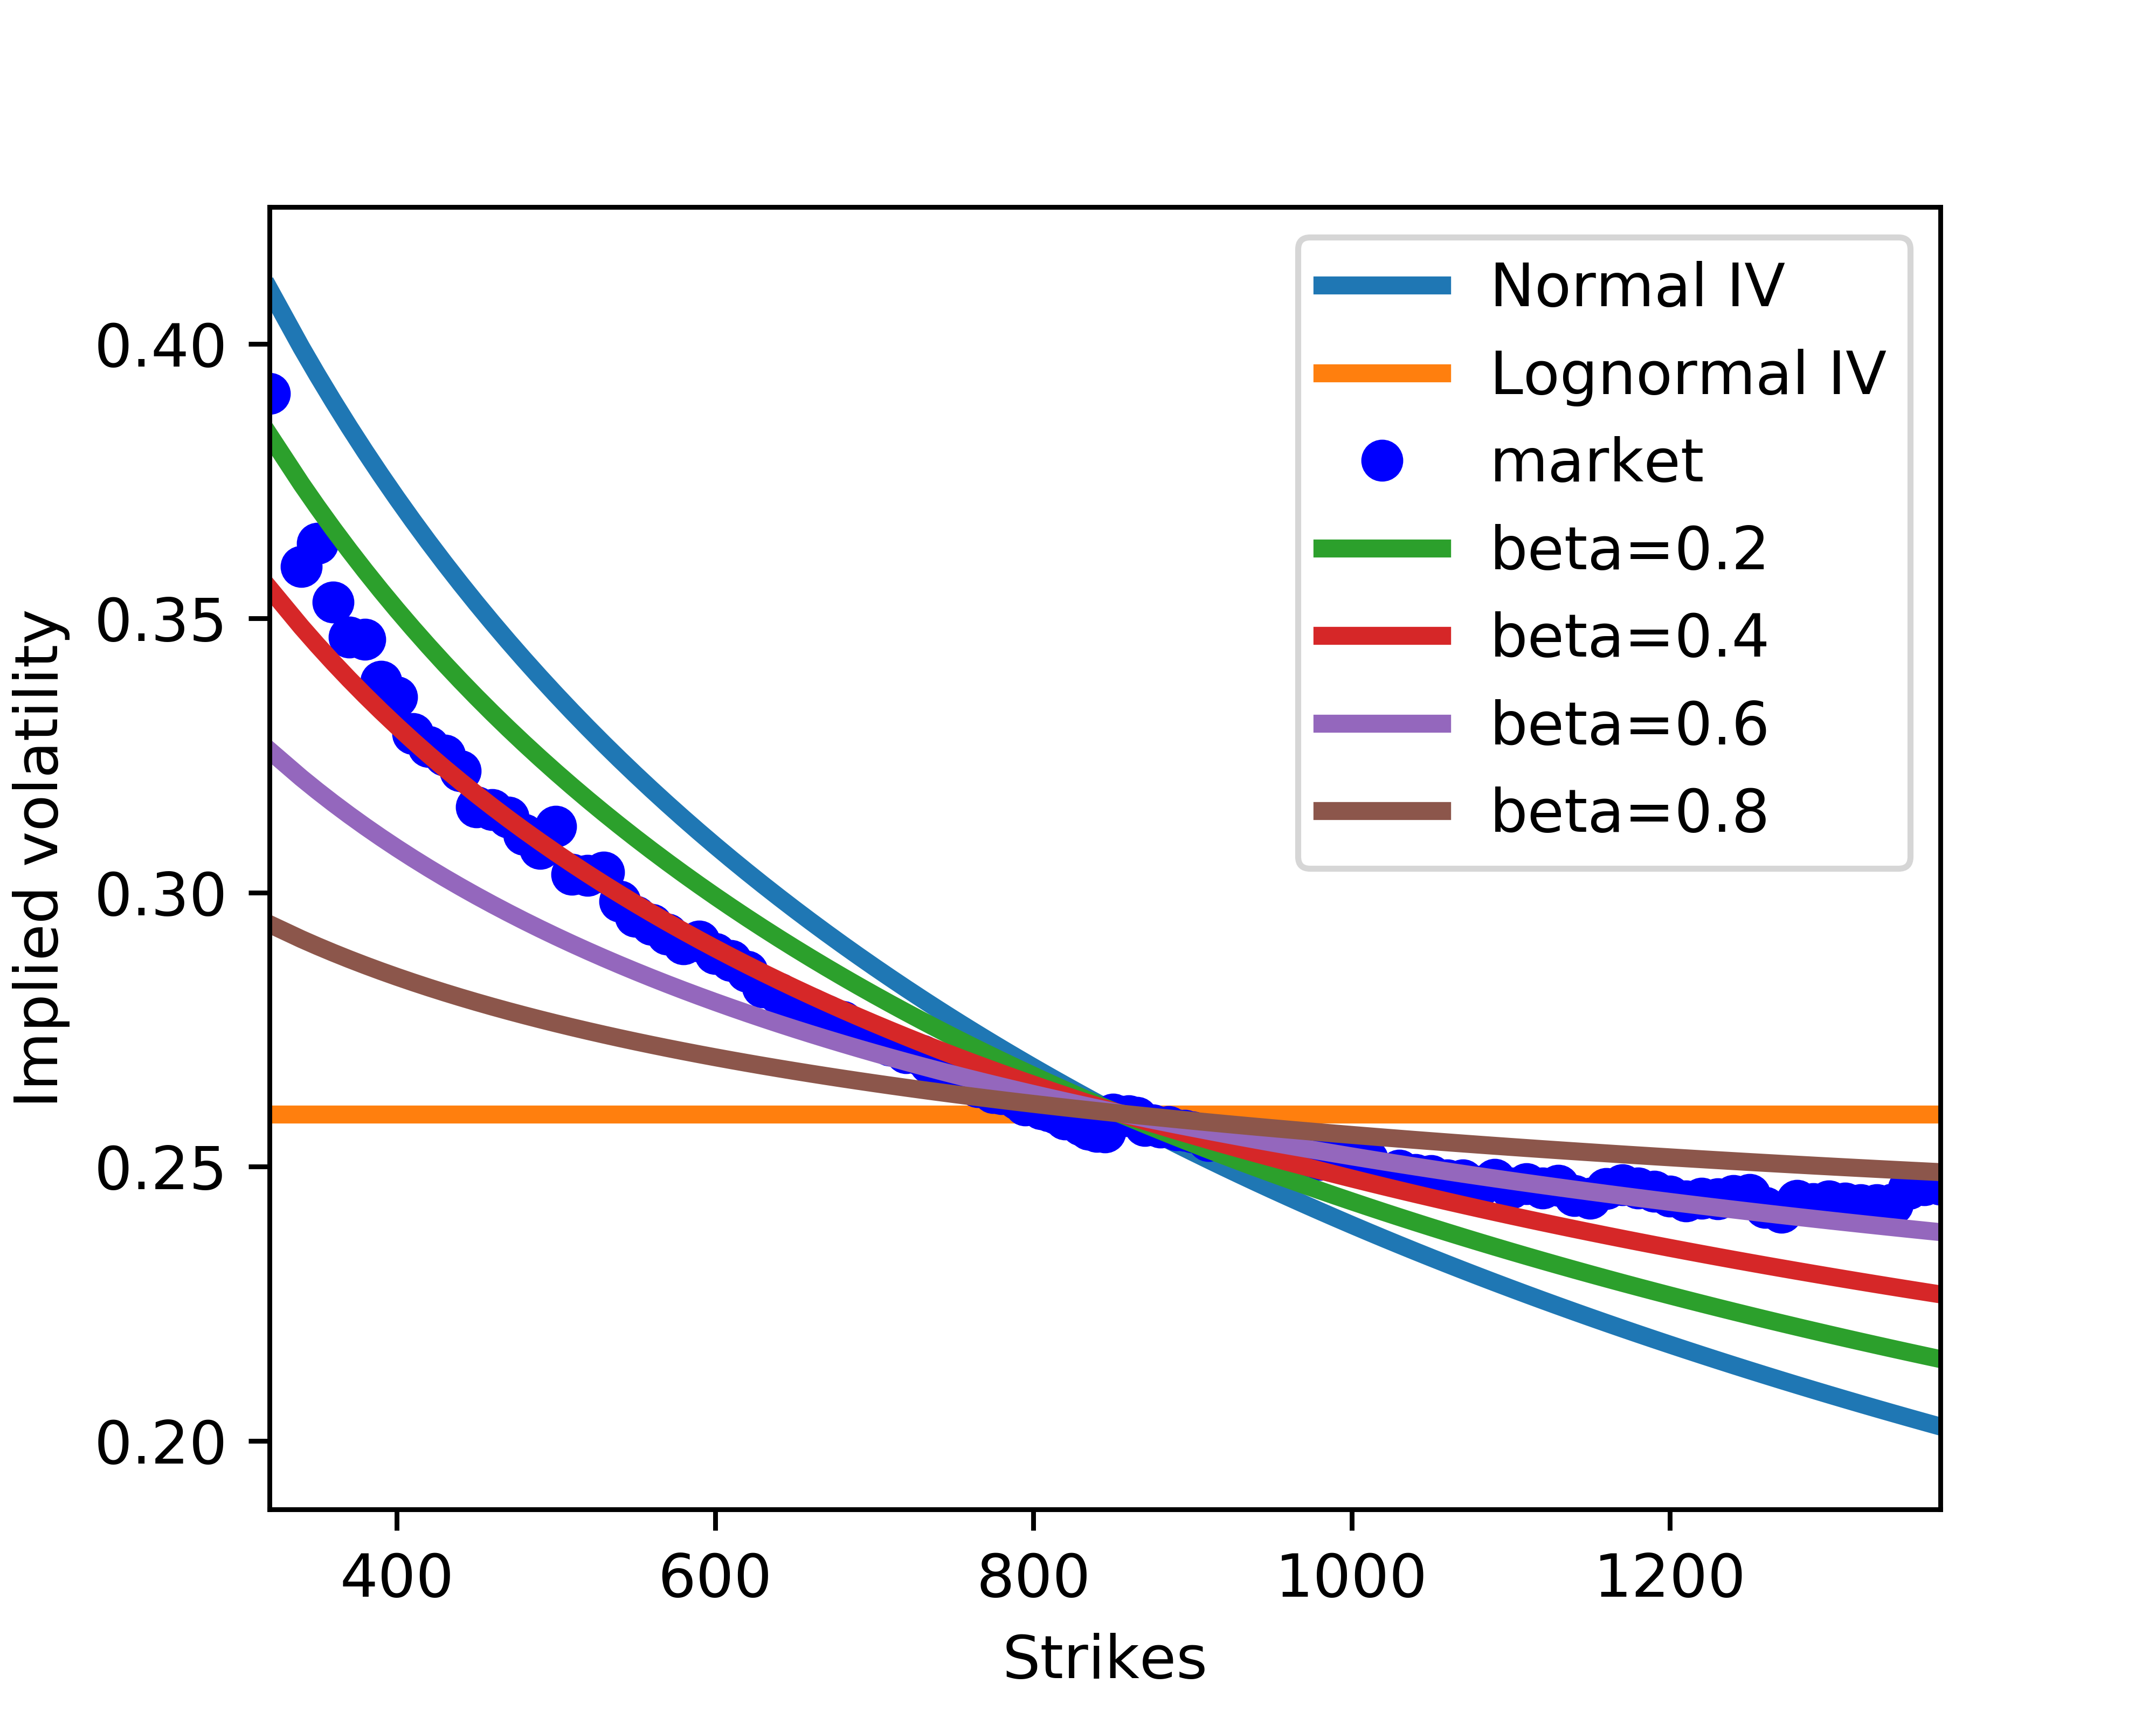
\includegraphics{DD}
	\caption{Displaced Diffusion}
\end{figure}

\noindent The displaced-diffusion model can be regarded as the weighted average of a lognormal and a normal model. $\beta$ can be regarded as the weights of the lognormal and normal model in displaced-diffusion model. When $\beta$ is equal to zero, the whole displaced-diffusion model becomes a normal model. When $\beta$ is equal to 1, the whole displaced-diffusion model becomes a lognormal model. When we change $\beta$ between 0 and 1, we are making “tradeoff” between a lognormal and a normal model. When the value of $\beta$ is close to 1, the line drawn in the chart is close to the lognormal model line, which is a horizontal line. When the value of $\beta$ is close to 0, the line drawn in the chart is close to normal model. 

\subsection{SABR Model}

\begin{figure}[ht]\centering
	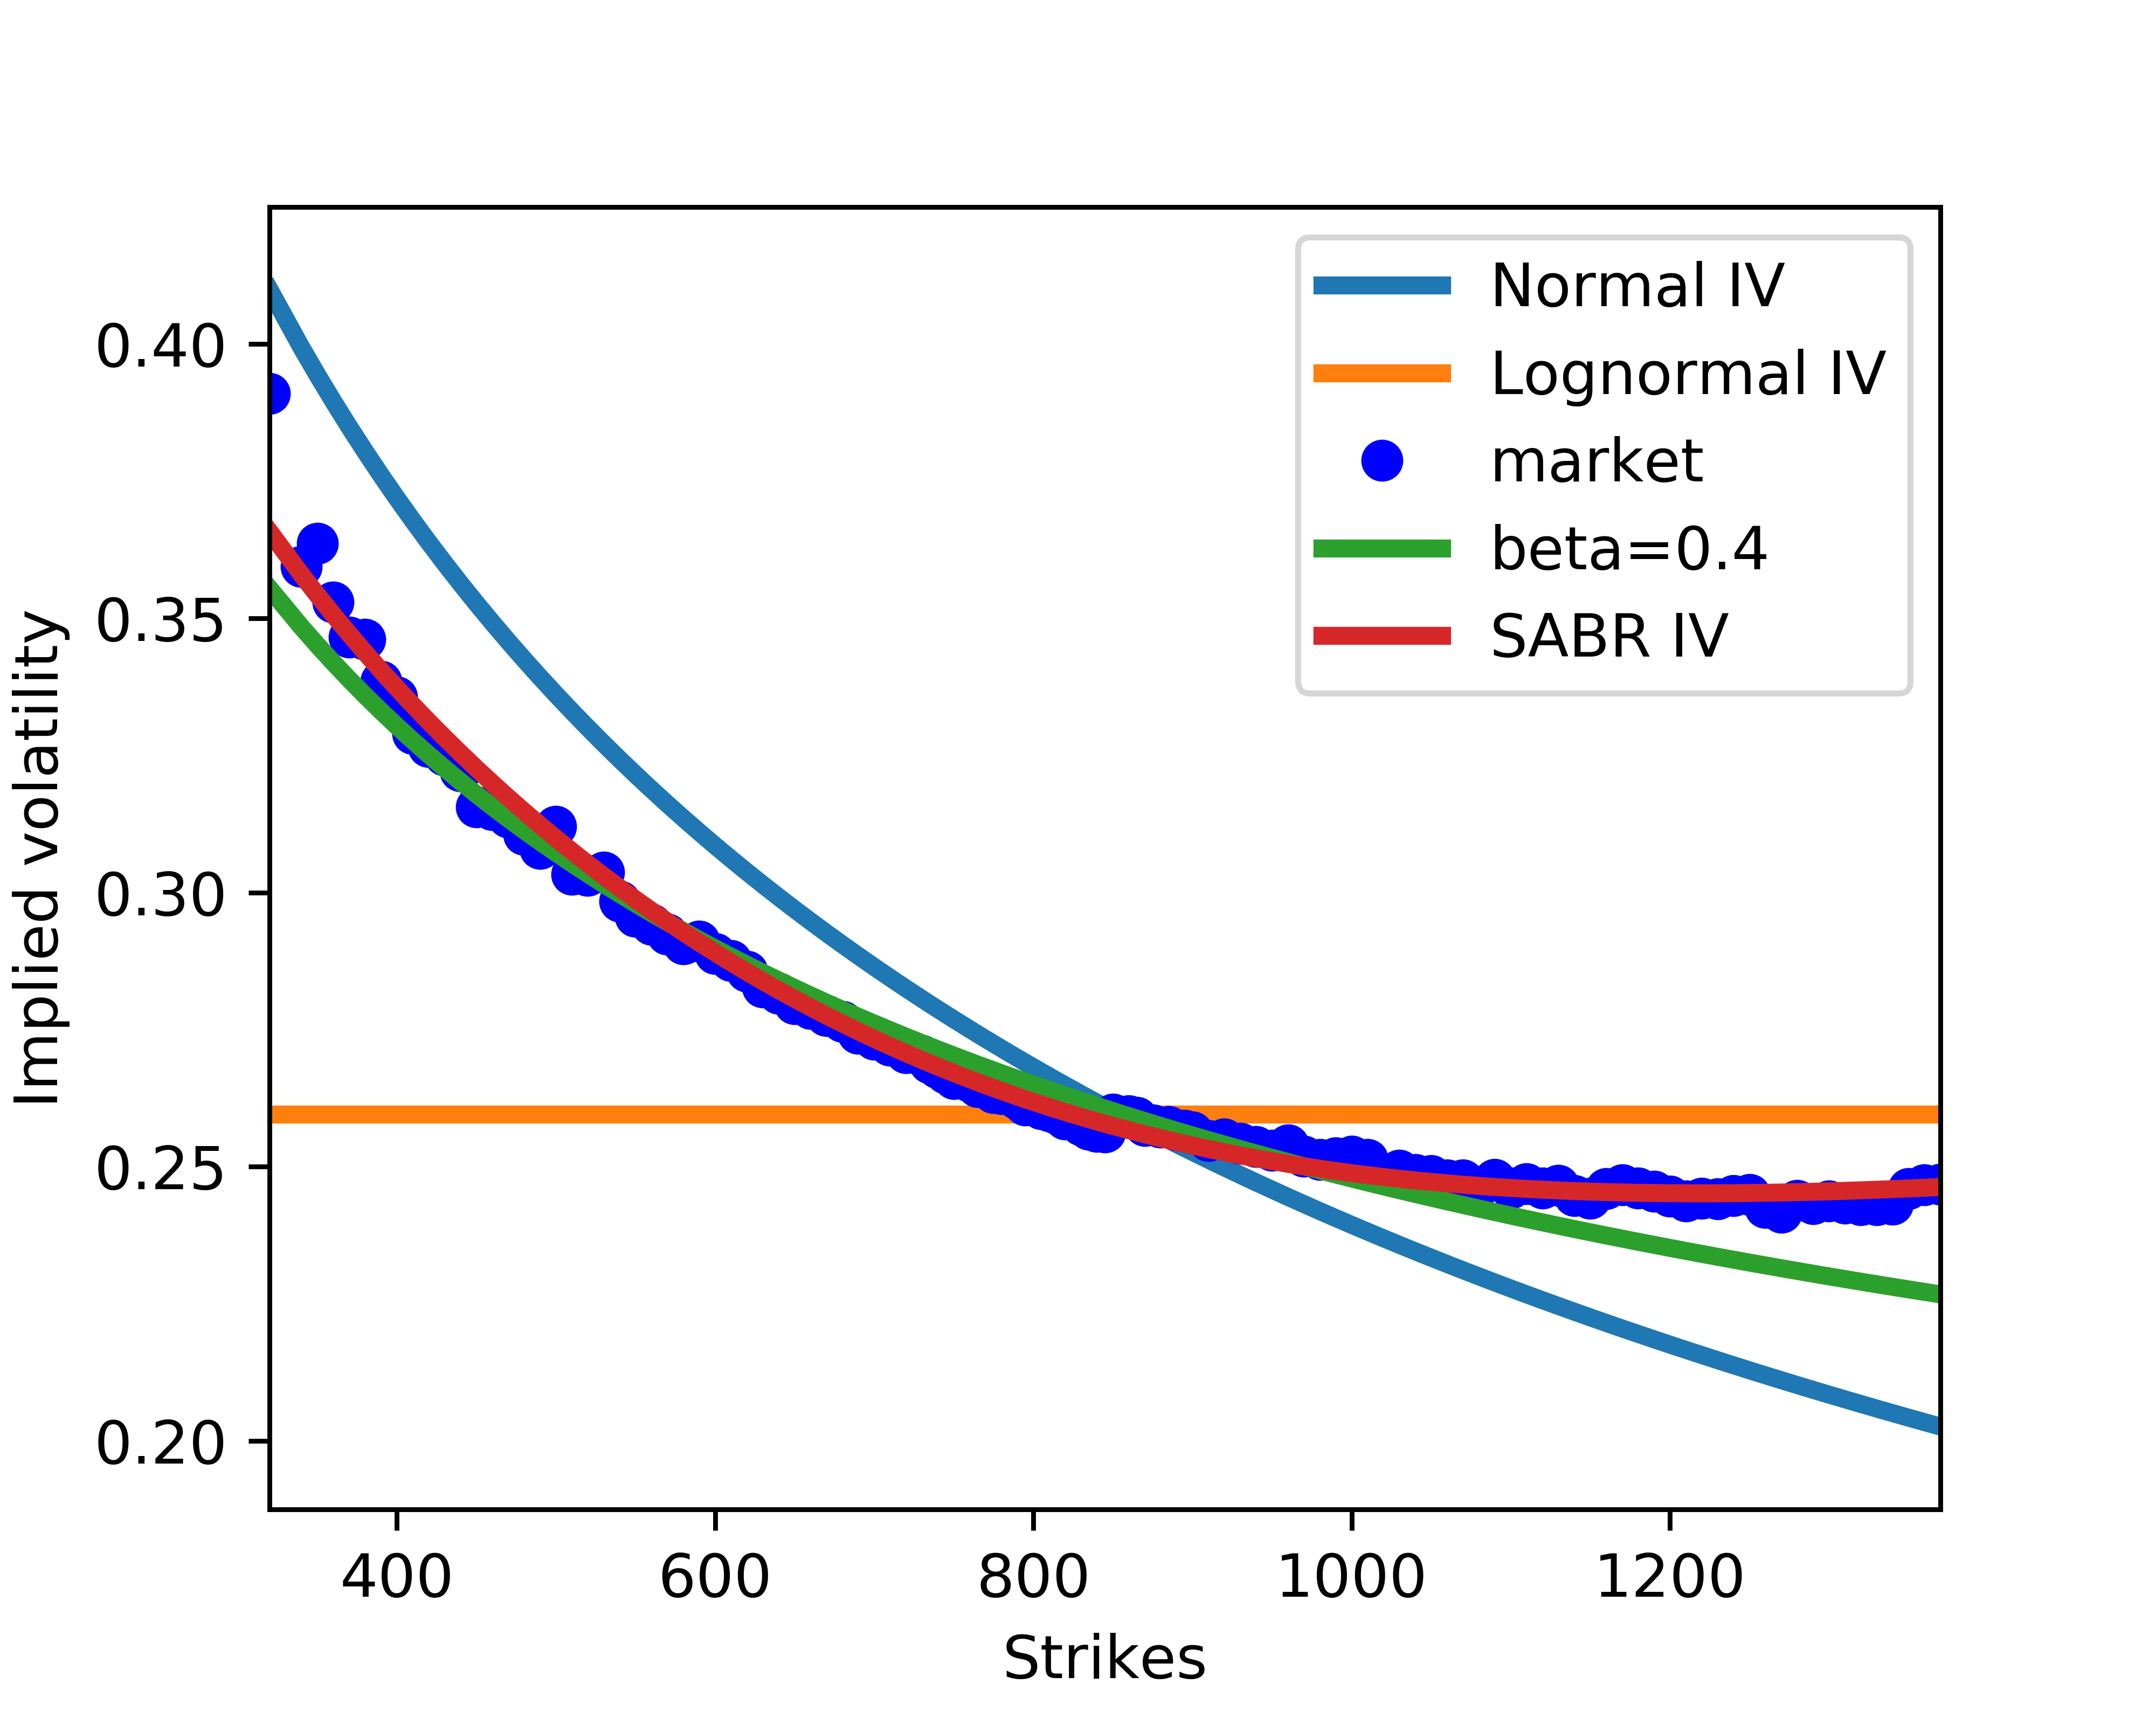
\includegraphics{SABR}
	\caption{SABR}
\end{figure}

\noindent In SABR Model, the correlation parameter $\rho$ is proportional to the skewness of stock returns. Positive correlation between stock and volatility will give us the return distribution with positive skewness. On the contrary, negative correlation between stock and volatility will give us the return distribution with negative skewness. In this case, when $\rho$ is negative, the curve is downward sloping and steep for the reason that negative correlation increases the price of out-of-money put options and at the same time, decreases the price of out-of-money call options. When $\rho$ is positive, the curve is more flattened. 

\noindent $\nu$ is called volatility of volatility in SABR Model. It is related to the kurtosis of stock return. When $\nu$ increases, the kurtosis of the stock return also increases. When $\nu$ is 0, the volatility is deterministic. When it comes to the curve, the increasing $\nu$ will move the right tail and left tail of the curve upward for the reason that larger volatility of volatility increases the price of out-of-money call options as well as the out-of-money put options. 

\section{Static Replication}

\noindent Payoff function: $h(S_T)=S_T^3+2.5\log{S_T}+10.0$

\subsection{Black Scholes Model - Payoff Function}
\noindent Under Black Scholes stock price process,
$$S_T=S_0 e^{(r-\frac{\sigma^2}{2})T+\sigma W_T}$$
$$S_T^3=S_0^3 e^{3(r-\frac{\sigma^2}{2})T}$$
$$\log{S_T}=\log{S_0}+(r-\frac{\sigma^2}{2}) T+\sigma W_T$$

\noindent Using risk free rate as the numeraire and given $B_0=0$ $B_T=e^{-rT}$
$$\frac{V_0}{B_0}=E^{Q^*}\left[\frac{V_T}{B_T}\right]$$
$$V_0=e^{-rT}E\left[V_T\right]=e^{-rT}\left[S_0^3 e^{3T(r-\frac{\sigma^2}{2})
}E\left[e^{3\sigma W_T}\right]+2.5\left[(r-\frac{\sigma^2}{2})T+\log{S_0}\right]+10\right]$$

$$=e^{-rT}\left[S_0^3 e^{3T(r+\sigma^2)}+2.5\left[(r-\frac{\sigma^2}{2})T+\log{S_0}\right]+10\right]$$

\noindent Inserting $\sigma_{ATM}=0.26$ and $S_0,r,T$, we are able to calculate $\bf{V_0=813409453.499285}$

\subsection{Bachelier Model - Payoff Function}
\noindent Under Bachelier stock price process,after some derivaton, we are able to get the value of payoff as:
$$V_0=S_0^3+3\sigma^2 S_0^3T+2.5\left[
\log{S_0}+\frac{1}{\sqrt{2\pi}}\int_{x^*}^{\infty}\log(1+\sigma \sqrt{T}x)e^{-\frac{x^2}{2}}dx\right]+10$$
\noindent where $x^*=\frac{-1}{\sigma \sqrt{T}}$ and \\
\noindent python calculates $\bf{V_0=773441382.5428648}$ by using $\sigma_{ATM}$ as the input\\

\subsection{Static Replication - Payoff Function}
\noindent We used single value of $\sigma_{ATM}$ as the input for derivative valuation for the above two scenarios. We can also value the derivative by static-replicating option available in the market.


$$V_0=e^{rT}E\left[h(S_T)\right] $$
$$=e^{-rT}h(F)+\int_{0}^{F}h^{''}(K)P(K)dK+\int_{F}^{\infty}h^{''}(K)C(K)dK$$

\noindent where $h'(S_T)=3S_T^2+\frac{2.5}{S_T}, h^{''}(S_T)=6S_T-\frac{2.5}{S_T^2}, F=S_0e^{rT}$
By setting strike price K as a random variable whose value is used as input for implied vol calculated by calibrated SABR, we are able to value the derivative by integrating the static-replication formula above. The value we obtained is $\bf{805098821.1389331.}$\\


\noindent``Model-free" integrated variance:
$$\sigma_{MF}^2 T=E\left[\int_{0}^{T}\sigma_t^2 dt \right]$$

\subsection{Black Scholes Model - "Model-Free" Integrated Variance}
\noindent Under Black Scholes, since it is model-free, we can just use $\sigma_{ATM}$ as the input on the left hand side of the equation to calculate integrated variance. The value calculated is $\bf{0.093528767.}$ Alternatively, we can do static-replication using right hand side to verify our result.
$$\left[\int_{0}^{T}\sigma_t^2 dt\right]=2e^{rT}\int_{0}^{F}\frac{P(K\	)}{K^2}dK+2*e^{rT}\int_{F}^{\infty}\frac{C(K)}{K^2}dK$$

The result of static replication is $\bf{0.093215189}$, quite close to what we get by just using $\sigma_{ATM}$.\\

\subsection{Bachelier Model - "Model-Free" Integrated Variance}
Under Bachelier, we use the same $\sigma_{ATM}$ and arrive at the same integrated variance of $\bf{ 0.093528767}.$\\

\subsection{Static Replication - "Model-Free" Integrated Variance}
Similar to what have been done in 3.3, we can let implied vol computed from SABR be dependent of strike price and integrate the formula below:
$$\left[\int_{0}^{T}\sigma_t^2 dt\right]=2e^{rT}\int_{0}^{F}\frac{P(K)}{K^2}dK+2e^{rT}\int_{F}^{\infty}\frac{C(K)}{K^2}dK$$
The value of integrated variance is $\bf{0.103380242}$ by applying static replication.

\section{Dynamics Hedging}

\begin{figure}[ht]\centering
	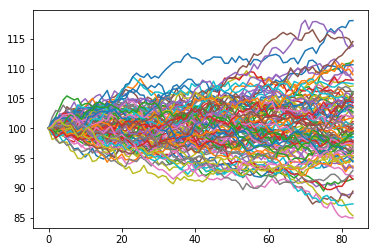
\includegraphics{Brownian}
	\caption{Brownian Motion}
\end{figure}

\begin{figure}[ht]\centering
	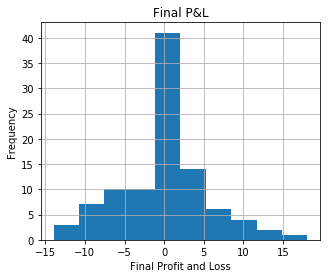
\includegraphics{PL}
	\caption{Profit and loss}
\end{figure}

Using the Black-Scholes formula, we can calculate the “fair” value of the option price. When the hedger uses dynamic hedging to rehedge continuously, the difference between the option value from Black-Scholes formula and the actual option value, which is the difference between the stock price and strike price at time t, should be zero. However, if the replication strategy deviates from the Black-Scholes method, the difference between the stock price and the strike price at time t may deviate from zero. The accumulated difference between the “fair value” from the Black-Sholes formula and the actual option value is the final profit and loss. According to the charts, if we rehedge a large number of times, the mean of the final profit and loss is 0. Moreover, the distribution of the final profit and loss is a normal distribution. Furthermore, when we hedge more frequently, the standard deviation decreases.

\bibliographystyle{\mystyle}   % 
\bibliography{myrefs}       % expects file "myrefs.bib"
\end{document} 